\documentclass[conference]{IEEEtran}
\IEEEoverridecommandlockouts
% The preceding line is only needed to identify funding in the first footnote. If that is unneeded, please comment it out.
\usepackage{cite}
\usepackage{amsmath,amssymb,amsfonts}
\usepackage{algorithmic}
\usepackage{graphicx}
\usepackage{textcomp}
\usepackage{xcolor}
\usepackage{pgfplots}
\usepackage{placeins}

\pgfplotsset{compat=1.18}

\def\BibTeX{{\rm B\kern-.05em{\sc i\kern-.025em b}\kern-.08em
    T\kern-.1667em\lower.7ex\hbox{E}\kern-.125emX}}
\begin{document}

\title{Video License Plate Parking System}

\author{\IEEEauthorblockN{Dominik Schweigl}
\and
\IEEEauthorblockN{Daniel Wenger}
\and
\IEEEauthorblockN{Nikola Adzic}
}

\maketitle

\section{Introduction}
Efficient parking management is an increasingly important challenge in urban environments, where traditional ticket-based parking systems often lead to congestion at entry and exit points, operational overhead, and poor user experience due to lost tickets and limited real-time visibility into parking availability.

This project presents a distributed, ticketless parking system based on automatic license plate recognition. Cameras installed at parking lot entry and exit points capture vehicle license plates, which serve as the identifier for access control and payment. This enables vehicles to enter and exit without physical tickets or manual interaction.
Users interact with the system through a single web application, accessible both on smartphones and on on-site payment stations, which allows them to pay, reserve parking spaces, view parking space availability, and discover the nearest parking facilities based on their location.

This work focuses on the system architecture, communication patterns, 
and deployment considerations of the distributed parking solution. 
Physical devices such as cameras, gates, and traffic lights are 
simulated, and license plate recognition is implemented using a 
YOLO license plate detection model combined with the EasyOCR optical character recognition model without evaluation 
of computer vision performance.

The remainder of this paper is structured as follows. Section~\ref{sec:system_architecture}
describes the overall system architecture and its main components. 
Section~\ref{sec:implementation_details} details the implementation 
of the edge, cloud, and web layers. Section~\ref{sec:evaluation} evaluates the system 
under different load scenarios. Section~\ref{sec:limitations} discusses 
the limitations of our system, and Section~\ref{sec:conclusion} summarizes the paper and outlines future work.

\section{System Architecture}
\label{sec:system_architecture}

The proposed parking system adopts a distributed edge--cloud architecture, 
organizing responsibilities across four distinct layers. The IoT layer 
handles sensing and actuation, the edge layer manages real-time processing 
and actuator control, the cloud layer provides centralized services for 
information management, booking, and payments, and the presentation layer 
enables user interaction through a web-based interface. This layered approach 
ensures low-latency parking actuator control at parking facilities while 
supporting centralized payment processing and a global view of parking 
availability. Figure~\ref{fig:architecture_diagram} illustrates the system 
components and their interactions. For simplicity, only a single parking 
lot is shown, though each facility deploys its own identical edge configuration.

\begin{figure}[t]
    \centering
    \includegraphics[width=1\linewidth]{assets/architecture_diagram.png}
    \caption{
        The architecture diagram for this project. For clarity, only 
        one parking lot edge is shown. Each parking lot has its own 
        edge server, gate, camera, and message queue.    
    }
    \label{fig:architecture_diagram}
\end{figure}

\subsection{Edge Layer}

Each parking lot is equipped with an edge server that is directly connected 
to the physical infrastructure of the facility. This includes two cameras 
positioned at the entry and exit gates, barrier gates, and traffic lights. 
The cameras continuously stream video data to the edge server via a local 
NATS message queue, which decouples video producers from consumers. 

The edge server performs real-time license plate detection on incoming video 
frames using a YOLO license plate detection model combined with the EasyOCR optical character recognition model. 
When a vehicle is detected at the 
entry gate, 
the edge server registers the vehicle locally and issues a command via the local
NATS message queue to open 
the entry barrier actuator. Local persistence using an SQLite database is maintained 
to ensure data robustness against temporary edge server failures.

At the exit gate, the edge server again detects the vehicle's license plate 
and queries the cloud backend to verify the payment status associated with 
the plate. If the vehicle has paid and the allowed exit window has not 
expired, the edge server opens the exit gate and signals a green traffic 
light. Otherwise, the gate remains closed and a red signal instructs the 
driver to return and complete payment. In addition, the edge server sends
occupancy updates to the cloud every time a vehicle enters or exits the parking lot.

\subsection{Cloud Layer}

The cloud backend is hosted on Amazon EC2 and implemented using the Akka 
framework. It serves as the central coordination point for all parking 
facilities. The cloud maintains global state such as parking lot registrations, 
current occupancy levels, payment status, and advances bookings to the
respective edge servers. Each parking 
lot periodically reports its current occupancy to the cloud, allowing the 
backend to maintain an up-to-date view of available parking spaces across 
all facilities.

The Communication between edge servers and the cloud backend uses a combination 
of synchronous and asynchronous mechanisms. REST-based HTTP endpoints exposed 
via Akka HTTP are used for operations from the edge to the cloud since many
operations need immediate responses, such as payment verification at exit gates. 
Asynchronous messaging via a 
NATS message queue hosted on it's own EC2 instance is used for event-driven interactions, such as propagating 
booking requests from the cloud to the appropriate edge server.


\subsection{Web and User Interaction Layer}

User interaction with the system is provided through a web application
implemented using React and hosted 
on a separate EC2 instance using Nginx as a web server. The same web 
application is accessible both from users' personal smartphones and from 
on-site payment stations within parking facilities. Through this interface, 
users can view available parking lots, reserve parking spaces in advance using 
their license plate number, complete payments, and discover nearby parking 
facilities based on their current location.

\section{Implementation details}
\label{sec:implementation_details}

This section presents the implementation of the system across its various 
layers, including the IoT components, edge server, cloud backend, and web 
interface. For each layer, the chosen design and implementation decisions 
are explained and justified.


\subsection{IoT Implementation}

The IoT components of the parking lot system are implemented in Python 
and deployed using Docker containers with \texttt{docker-compose}, ensuring 
that the system is independent of the underlying execution infrastructure. 
Both the camera simulations and actuator interfaces run inside these 
containers.

\paragraph{Camera}
The entry and exit points of the parking lot are simulated by two camera 
streams, which alternately transmit images from a car license plate detection 
dataset and a reference empty street scene. 
The dataset we use is the Car License Plate Detection dataset from 
Kaggle. It features more than 400 images of car front/ rear views 
with clearly visible license plates. We chose a subset of the 50 most clearly
visible license plates for our simulation.

Images are published to an edge server via a NATS message queue via the 
camera simulation python script to two separate message queue subjects. 
It is made sure that the data sent 
by the entry and exit camera streams is consistent. This means that the exit 
camera will only show cars leaving that have previously entered. The 
duration of the cars inside the car parks is sampled randomly.

Cars enter the lot at a steady pace, with one car added every two display cycles of 3 seconds (\texttt{FRAME\_DELAY}), yielding an average entry rate of
\[
R_\text{entry} = \frac{1}{2 \cdot \text{FRAME\_DELAY}} \approx 0.166 \text{ cars/second}.
\]
Each car has a probability of leaving the lot in any given frame of
\[
P_\text{exit} = \frac{1}{4 \cdot \text{FRAME\_DELAY}} \approx 0.0833 \; (8.33\%),
\]
corresponding to an average exit rate of
\[
R_\text{exit} = \frac{P_\text{exit}}{\text{FRAME\_DELAY}} \approx 0.028 \text{ cars/second}.
\]
This setup results in a parking lot that gradually fills over time, where entries outpacing exits.

\paragraph{Parking Lot Gates and Traffic Light Interface}
The parking lot gates and traffic lights are simulated via a web-based 
interface implemented using \texttt{FastAPI}. The framework was selected 
due to its support for rapid and intuitive development. In addition, 
FastAPI provides native support for asynchronous 
communication and WebSockets, which makes it well suited for real-time 
IoT applications.

The interface provides a live view of the current state of all actuators 
for each parking lot individually. It receives continuous state updates 
from the edge server through the local NATS message broker, ensuring that 
changes in actuator states, such as barrier positions or traffic light 
signals, are reflected on the web dashboard. Furthermore, the 
interface displays the camera streams from the entry and exit points, 
which allows to visually monitor the camera streams and correlate actuator 
behavior with observed traffic conditions.

\subsection{Edge Implementation}

The edge server is responsible for all real-time processing at the parking 
lot gates. For each incoming camera frame, it executes a YOLOv11-based license 
plate detection pipeline followed by optical character recognition (OCR) to 
extract the license plate text. All detections are processed locally at the 
edge without requiring immediate interaction with the cloud. This design 
keeps network traffic to the cloud low and
ensures low-latency actuator control and allows the system to remain 
operational during temporary cloud disconnections, though with some limitations 
at the exit gate due to synchronous payment verification at the cloud. The edge server is 
implemented in Python, as the employed machine learning models and inference 
pipelines are exclusively available through Python-based frameworks.

The edge deployment follows the same container-based approach as the IoT layer.
Both the edge server and the local NATS message broker are executed within 
Docker containers, and together with the IoT components they are deployed 
as a single edge application using \texttt{docker-compose}. This setup 
enables consistent and reproducible
deployment across different parking facilities, simplifies configuration
management, and allows the complete edge stack—including processing logic and
messaging infrastructure—to be started, stopped, and updated as a single unit.

To maintain local state, the edge server uses a lightweight SQLite database. 
SQLite was selected for its low operational overhead, zero-configuration 
deployment, and suitability for resource-constrained edge environments. As 
an embedded database, it runs within the application process and requires no 
separate database service, providing sufficient performance for handling 
several hundred concurrent parking sessions per lot while keeping the system 
simple.

When a vehicle appears at the entry point, the edge server checks whether an 
active session for the same license plate already exists and only creates a 
new record if the vehicle is not already inside the parking lot. This prevents 
duplicated entries caused by repeated detections of the same vehicle while it 
remains in front of the entry camera. For exit events, the edge queries the cloud 
service to verify the payment status, retrieves the corresponding local 
session from SQLite, and completes it by recording the exit timestamp.

Communication between the camera streams, actuator controllers, and the edge 
server is handled using NATS as the message broker. NATS was selected for its 
lightweight architecture, low-latency message delivery, and minimal operational 
overhead, making it well suited for deployment on resource-constrained edge 
servers. In contrast to heavier brokers such as Apache Kafka or RabbitMQ, which 
emphasize message persistence and complex broker management, NATS is optimized 
for real-time, transient messaging patterns while the throughput and provides 
ample throughput to reliably handle the modest message rates in the low tens 
generated by the camera streams and actuator commands.

Using NATS creates a clean decoupling between data producers (camera streams) 
and consumers (edge processing and actuator controllers).
The camera streams publish data using NATS core publish--subscribe semantics, 
where messages are delivered on a best-effort basis only to currently active 
subscribers and are not persistently stored. This behavior aligns with the 
nature of camera frames, which are only relevant at the time of generation 
and have no value if processed later. By avoiding message persistence, the 
system reduces memory and storage overhead while ensuring timely delivery of 
live camera data. Actuator commands and state updates similarly benefit from 
this low-latency, ephemeral communication model, enabling responsive and 
reliable gate control at the edge.


\subsection{Cloud Implementation}

In the cloud layer we rely on Akka Typed as the central orchestration 
mechanism for all parking-lot related functionality. An embedded Akka 
HTTP server runs within the same ActorSystem and exposes a 
synchronous HTTP REST API to edge servers and the web application. 
This is a standard protocol, which makes it easy to provide uniform access
for edge servers and web clients alike. Internally, the system is entirely 
message-driven, which provides clear separation of concerns and concurrency.

\begin{figure}[h]
    \centering
    \includegraphics[width=1\linewidth]{assets/actor_structure.png}
    \caption{
        Structure of the application-level Akka actor hierarchy in the cloud backend.
        The user actor is shown as the root of the application-level actors,
        Akka system and infrastructure actors are omitted for clarity.
    }
    \label{fig:actor_structure}
\end{figure}

At the core sits a typed ParkingLotManager actor that maintains the 
registry of parking lots and supervises one ParkingLot actor per lot. 
The manager accepts commands to register and deregister lots, to update 
occupancy, and to fetch either the status of a specific lot or the 
complete set of registered lots. Each ParkingLot actor keeps the local 
state for a single lot. Parking lot edge occupancy updates 
are handled as fire-and-forget messages to minimize latency, while status 
queries are served using Akka's ask pattern.

Payments are handled by a dedicated typed Payment actor that tracks a 
parking session per license plate. When a car is recorded as having 
entered, the actor creates or updates the session with the entry time. 
A payment command marks the session as paid and computes the price based 
on the parking duration using a simple policy with half-hour increments. 
At exit, the actor can be asked synchronously to verify whether the car 
has paid and to return the current price; once the car leaves, the 
session is deleted to ensure that only currently parked cars are stored,
which reduces system load.

Bookings are mediated by a Booking actor that acts as the 
cloud-side gateway to the edge servers. When a booking is created 
through the API, the actor publishes a to a parking-lot 
specific NATS subject, which the corresponding edge server subscribes 
to. This approach decouples the cloud from the physical 
deployment of edge servers, allowing bookings to be routed while
the edge network locations transparent to the cloud. When a 
booking is cancelled, the actor similarly publishes an 
action “cancel” message. By using an asynchronous message queue, 
the system remains resilient to temporary connectivity issues. This approach intentionally keeps booking 
state lightweight in the cloud and delegates the effective reservation 
and occupancy enforcement to the edge, where the real-world constraints 
such as maximum occupancy and gate control are managed. The edge server 
is therefore responsible for enforcing bookings locally and rejecting 
incoming vehicles when all available parking spaces are already reserved.

For the computation of the closest parking lots based on user location,
the cloud backend defines a Routing Actor that calculates the
Haversine distance between the user's coordinates and each parking lot's
stored geographical location. The actor then sorts the parking lots
based on this distance and returns the sorted list to the web client.

\subsection{Web Interface}

For the web interface, we implemented a web application using React that allows
users to interact with the parking system. Through this application, users can
see all registered parking lots, check their current availability, reserve
a parking space in advance by entering their license plate number and pay. 
React was chosen for its component-based architecture, which simplifies
the development and maintenance of dynamic user interfaces.
The interface was styled using Tailwind CSS, whose utility-first approach enables
rapid creation of responsive and consistent layouts with minimal custom styling.

To help users find a suitable parking lot, the application can access the
current location of the client device using the browser's geolocation feature.
Each parking lot is provided by the backend together with its geographical
coordinates and the distance to the corresponding parking lot. The frontend
application sorts the results so that nearby
parking options are shown first. A routing button is also provided, which opens
a navigation view in an external map service for the selected parking lot.

\section{Evaluation}
\label{sec:evaluation}

\subsection{Evaluation Setup}

The cloud components of the system were deployed on Amazon Web Services 
(AWS) using Terraform to ensure reproducibility and consistency across 
experiments. The setup consists of three EC2 instances hosting the 
backend application, message broker, and web frontend, respectively. 
All instances use the \texttt{t3.micro} instance type, providing 2 
virtual CPUs and 1~GB of RAM, which is sufficient for evaluating the 
system under moderate load. The instances run Amazon Linux 2023 (x86\_64).

The backend service is deployed as a Java-based Akka application running 
on Amazon Corretto JDK~17, while the NATS message broker is hosted in a 
Docker container to facilitate lightweight and isolated operation. The 
web frontend is served via Nginx as a static application. Network access 
is controlled using a dedicated security group that exposes only the 
required ports for HTTP communication, backend APIs, NATS messaging, 
and SSH access.


\subsection{Test Case 1: Cloud Backend Load under Realistic Edge Traffic}

This test case evaluates the scalability limits of the cloud backend
under a realistic workload generated by multiple independent edge
servers. In a real deployment, geographically distributed parking
facilities continuously send occupancy updates and sporadically trigger
payment-related requests. The goal of this experiment is to determine
up to which load level the cloud backend operates reliably and to
identify the saturation point at which latency and error rates increase
rapidly.

\subsubsection*{Workload Model}

To generate load, a custom asynchronous Python-based load generator was
used. Instead of issuing synthetic request bursts, the tool simulates
the behaviour of multiple independent edge servers:

\begin{itemize}
  \item Each simulated edge server periodically sends occupancy updates
        to the cloud backend.
  \item Request arrivals follow a Poisson process, reflecting the
        stochastic nature of real vehicle movements.
  \item In addition to occupancy updates, a low but constant rate of
        payment sessions is generated. Each payment session consists of
        multiple dependent HTTP requests (enter, check, pay, exit),
        modelling realistic user interaction rather than isolated
        requests.
  \item A global limit on the number of in-flight HTTP requests is
        enforced to prevent the client from unrealistically
        overwhelming the server.
\end{itemize}

This composition ensures that the observed behaviour reflects realistic
operational load rather than a purely synthetic stress test.

\subsubsection*{Experimental Setup}

The number of simulated edge servers was fixed at ten. The offered load
was increased step-wise by raising the occupancy update rate per edge
server, while keeping all other parameters constant. Each load level was
measured for 90 seconds following a warm-up phase of 10 seconds.

The following metrics were recorded:
\begin{itemize}
  \item Achieved total request throughput (requests per second)
  \item Success rate and number of timeouts
  \item End-to-end request latency, with a focus on the 95th percentile
\end{itemize}

\begin{figure}[t]
\centering
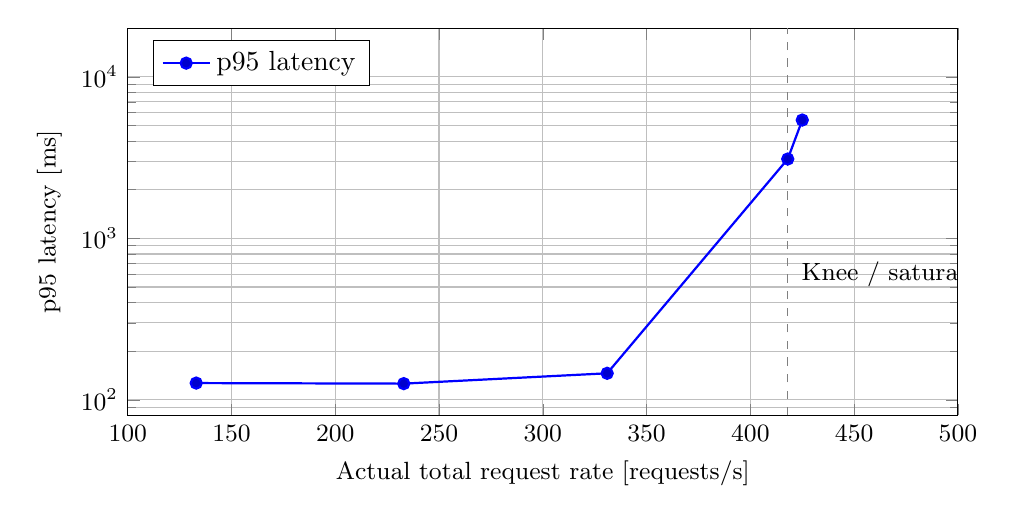
\begin{tikzpicture}
\begin{axis}[
    width=\linewidth,
    height=6.5cm,
    xlabel={Actual total request rate [requests/s]},
    ylabel={p95 latency [ms]},
    ymode=log,
    xmin=100, xmax=500,
    ymin=80, ymax=20000,
    grid=both,
    legend style={at={(0.03,0.97)},anchor=north west},
    tick label style={font=\small},
    label style={font=\small},
]

\addplot+[mark=*, thick]
coordinates {
  (133,127)
  (233,126)
  (331,146)
  (418,3098)
  (425,5400)
};
\addlegendentry{p95 latency}

% Knee annotation
\draw[dashed,gray] (axis cs:418,80) -- (axis cs:418,20000);
\node[anchor=west,font=\small] at (axis cs:420,600)
{Knee / saturation onset};

\end{axis}
\end{tikzpicture}
\caption{Cloud backend latency under increasing edge-generated load.
The system shows stable and low latency up to approximately
330~requests/s. At around 420~requests/s, tail latency increases
sharply, indicating the onset of saturation. Further load leads to
severe overload and queueing collapse.}
\end{figure}
\FloatBarrier
The results show three distinct operating regions. For low to moderate
load levels, the backend scales linearly and maintains a stable tail
latency below 200~ms. At approximately 420~requests/s, the system reaches
its saturation point, where latency increases by more than an order of
magnitude and timeouts begin to occur. Beyond this point, additional
load reduces the effective throughput and leads to severe degradation in
both latency and success rate, which is characteristic of overload in
queue-based systems.

\subsection{Test Case 2: Web Interface Load Test (Nginx + React)}
The goal of this test was to evaluate the performance of the web interface, 
specifically the ability of the Nginx server to serve a compiled React 
frontend under concurrent access. This test was 
intentionally isolated from the rest of the system components, meaning that 
neither the Akka cloud backend nor any edge servers were involved.

The web server was evaluated using a step-wise open-loop load test with \texttt{wrk2}. 
The test script incrementally increases a fixed target request rate (\texttt{-R}) while keeping
the number of threads and connections constant. Each step consists of a short warmup phase
followed by a measurement phase, during which achieved throughput is recorded.

Two endpoints were tested independently using identical parameters:
\begin{itemize}
  \item the root endpoint (\texttt{/})
  \item the largest JavaScript bundle served by the frontend
\end{itemize}

The achieved request rate is plotted against the configured target rate. 
Deviation from the ideal linear tracking behavior indicates saturation and marks the knee
of the system.

\begin{figure}[t]
\centering
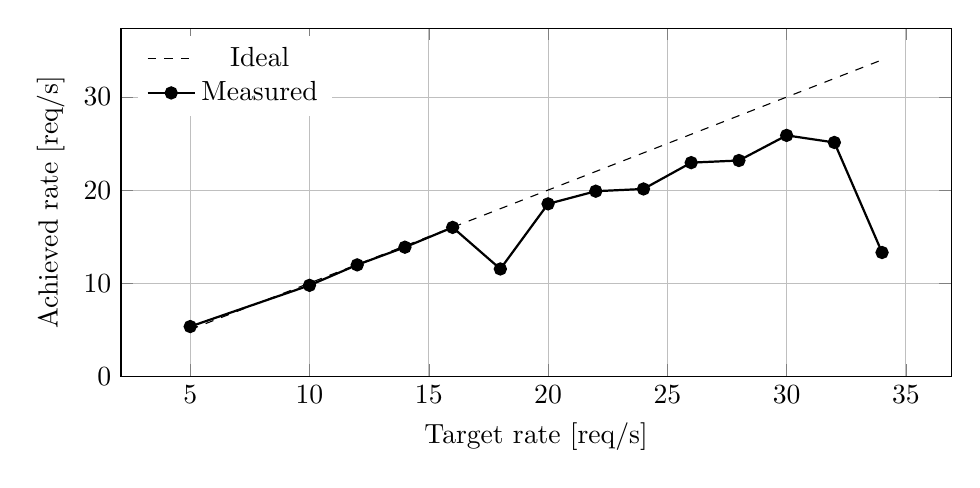
\begin{tikzpicture}
\begin{axis}[
  width=\linewidth,
  height=6cm,
  grid=both,
  xlabel={Target rate [req/s]},
  ylabel={Achieved rate [req/s]},
  ymin=0,
  legend style={at={(0.02,0.98)},anchor=north west,draw=none}
]

% Ideal tracking
\addplot[dashed] coordinates {
  (5,5) (10,10) (12,12) (14,14) (16,16)
  (18,18) (20,20) (22,22) (24,24)
  (26,26) (28,28) (30,30) (32,32) (34,34)
};
\addlegendentry{Ideal}

% Measured
\addplot[mark=*, thick] coordinates {
  (5,5.33) (10,9.76) (12,11.96) (14,13.86) (16,15.99)
  (18,11.52) (20,18.52) (22,19.88) (24,20.12)
  (26,22.95) (28,23.18) (30,25.88) (32,25.12) (34,13.29)
};
\addlegendentry{Measured}

\end{axis}
\end{tikzpicture}
\caption{wrk2 step test results for the root endpoint (\texttt{/}).}
\label{fig:wrk2-root}
\end{figure}

\begin{figure}[t]
\centering
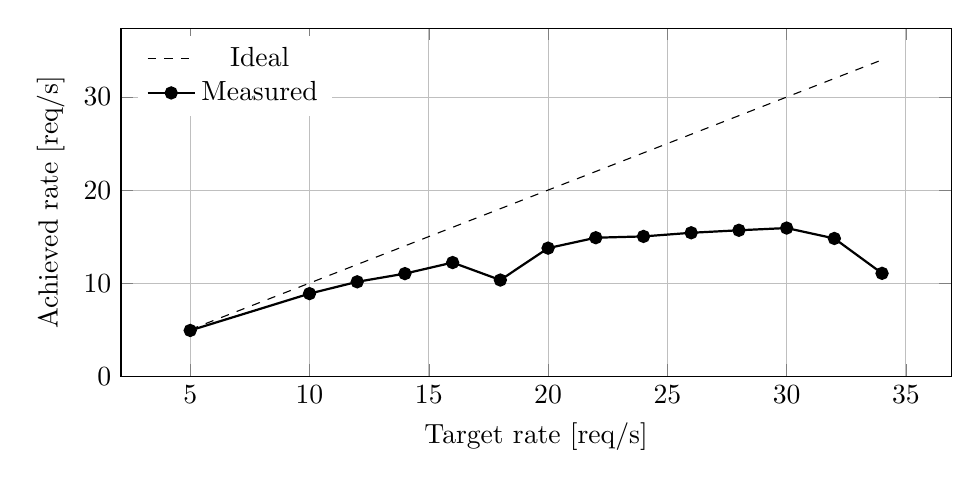
\begin{tikzpicture}
\begin{axis}[
  width=\linewidth,
  height=6cm,
  grid=both,
  xlabel={Target rate [req/s]},
  ylabel={Achieved rate [req/s]},
  ymin=0,
  legend style={at={(0.02,0.98)},anchor=north west,draw=none}
]

% Ideal tracking
\addplot[dashed] coordinates {
  (5,5) (10,10) (12,12) (14,14) (16,16)
  (18,18) (20,20) (22,22) (24,24)
  (26,26) (28,28) (30,30) (32,32) (34,34)
};
\addlegendentry{Ideal}

% Measured
\addplot[mark=*, thick] coordinates {
  (5,4.91) (10,8.87) (12,10.14) (14,11.02) (16,12.21)
  (18,10.33) (20,13.76) (22,14.88) (24,15.02)
  (26,15.41) (28,15.68) (30,15.92) (32,14.80) (34,11.05)
};
\addlegendentry{Measured}

\end{axis}
\end{tikzpicture}
\caption{wrk2 step test results for the largest JavaScript bundle.}
\label{fig:wrk2-js}
\end{figure}

Figures~\ref{fig:wrk2-root} and~\ref{fig:wrk2-js} plot the achieved request rate against the
configured target rate. The dashed line represents ideal linear behavior, where the server
fully tracks the offered load.

At lower request rates, both endpoints closely follow the ideal curve, indicating stable
operation without saturation. As the target rate increases, the measured throughput deviates
from linear scaling, marking the knee of the system.

The root endpoint maintains linear scaling up to a higher request rate, while the JavaScript
bundle reaches saturation earlier. This is expected due to the higher bandwidth and I/O
requirements of serving large static assets. Beyond the knee, increasing the offered load
does not result in higher throughput.

\section{Limitations}
\label{sec:limitations}


While the implemented system covers the core functionality of a video
license plate parking system, there are several limitations to consider.

\paragraph{Payment event latency optimization}
To reduce latency at the exit gate, payment events could be propagated 
to the edge server proactively rather than queried on demand. In the 
current design, the edge server performs a synchronous request to the 
cloud backend when a vehicle approaches the exit, introducing avoidable
latency. By pushing payment status updates to the edge immediately after 
a transaction is completed, the edge system could locally cache this 
information and eliminate the need for synchronous cloud queries at 
exit time. This approach would result in faster gate responses and 
improved robustness during transient cloud disconnections.

This limitation is further emphasized by the fact that the current 
payment system is a mock implementation without integration with real 
payment gateways. In a production environment, secure payment providers 
such as Stripe or PayPal would be required to process actual financial 
transactions, inevitably introducing additional latency during payment 
verification. By proactively propagating payment status updates to the 
edge server, this added delay could be mitigated.

\paragraph{Security and authentication}
Another major limitation of the current system is the absence of 
authentication and authorization mechanisms. At present, the cloud 
backend does not verify the identity of parking lot servers during 
registration or when receiving occupancy updates, which could allow 
unauthorized entities to inject or manipulate parking lot data. A 
production--ready deployment would therefore require the introduction 
of secure authentication mechanisms, such as mutual TLS or API 
key based access control, to ensure data integrity and system security.

\paragraph{Cloud Scalability and Availability}
A further limitation of the current system is the simplicity of the 
cloud deployment. The cloud components—the Nginx web server, 
the Akka-based backend, and the NATS message broker—are each hosted 
on a single EC2 instance, without load balancing or automatic scaling. 
While sufficient for prototyping and evaluation, this architecture may 
not sustain high traffic volumes and offers limited fault tolerance, 
as each component constitutes a single point of failure.
Reliability and scalability could be 
significantly improved by deploying the cloud services using 
container orchestration platforms such as Amazon ECS, in combination 
with load balancers and auto-scaling mechanisms. 

Furthermore, because all cloud-to-edge communication is mediated by 
the message broker and involves temporary buffering of messages, the 
system could benefit from brokers such as Apache Kafka, which provide 
persistent storage, replication, and message replay in the event of 
consumer or broker failures. For the scale of the current system, 
however, NATS remains a suitable choice. To prevent loss of critical 
messages, such as booking updates, when an edge server is temporarily 
disconnected, NATS JetStream could be employed to enable message 
persistence and reliable delivery.

\paragraph{Booking Race Conditions}
The current booking implementation does not prevent race conditions 
when web users and drivers at the entry gate attempt to access the 
last available 
parking space simultaneously. For example, a user may reserve the 
final space through the web interface at the same time a car arrives 
at the entry gate without a prior booking. If the car enters and 
the booking request arrives at the cloud before the edge server updates its occupancy, 
the booking request is still processed successfully by the cloud 
and forwarded to the edge, resulting in overbooking. To fully prevent 
such race conditions, the booking process would require explicit 
confirmation from the edge server before finalizing a reservation.

\paragraph{Deployment Automation}
The deployment process could benefit from greater automation. While 
the cloud infrastructure is provisioned using Terraform, the web 
application bundle and the Akka backend JAR currently need to be
built manually and locally, which are then automatically uploaded
during terraform deployment using file provisioners.
 This manual step introduces 
additional effort and increases the potential for human error, which can 
affect reproducibility and slow down iterative development.
Implementing 
a fully automated CI/CD pipeline, for example using, 
GitHub Actions, or GitLab CI, would streamline the build, test, and 
deployment processes. Such a pipeline could automatically compile the 
backend and frontend artifacts, run tests, and deploy them to the 
cloud infrastructure with minimal human intervention, improved 
reliability, and reduce deployment time.

\paragraph{Distance Calculation}
Nearby parking lots are currently identified using the Haversine formula, 
which computes straight-line distances. For more accurate routing, 
integration with a mapping service that provides real-world driving 
distances and directions would be advantageous, though it may introduce 
additional latency.

\paragraph{License Plate Detection Model}
In a production system, the detection model would ideally be fine-tuned 
to the specific environment and camera angles of the parking lot 
entrances. For this project, we employ a pre-trained YOLOv11 license 
plate detection model combined with EasyOCR for optical character 
recognition. In our scenario, this approach is sufficient to 
demonstrate the system's functionality, as each car is represented 
by a single, unchanging image, resulting in consistently stable 
detection outcomes.


\section{Conclusions and future work}
\label{sec:conclusion}

This paper presented a distributed, ticketless parking system based on 
automatic license plate recognition, combining edge computing, 
cloud-based coordination, and a web-based user interface. By processing 
camera streams locally at the edge and delegating global state management, 
payments, and bookings to a cloud backend, the system achieves low-latency 
gate control while maintaining a centralized view of parking availability. 
The actor-based cloud architecture, NATS messaging, and 
containerized deployment demonstrate a scalable and modular design 
suitable for coordinating multiple parking facilities. Experimental 
evaluation shows that the system performs reliably under moderate load, 
with stable response times for cloud APIs, web access, and edge messaging.

Several limitations remain and point toward future work. Payment 
verification currently introduces avoidable latency at the exit gate 
and could be optimized through proactive propagation of payment events 
to the edge. Security mechanisms such as authentication and authorization 
are not yet implemented and would be essential in a production deployment. 
Cloud scalability and fault tolerance are limited by single-instance 
components and could be improved through load balancing, auto-scaling, 
and persistent messaging solutions. Additional challenges include booking 
race conditions, partial deployment automation, simplified distance 
calculations, and the use of a pre-trained license plate detection model 
without environment-specific tuning. Addressing these aspects would 
further improve robustness, scalability, and real-world applicability 
of the proposed system.

\end{document}
